In a gesture to have a general idea about the distribution of cycling levels, we turn to standard power profile and use the average cycling pace to plot the power curve. The dataset includes the riders' maximum power output during a certain period of time, ranging from novice to world-class, both men and women. Also, the power profile chart gives out the standard of different types, ensuring us to analyze the ability of riders in all domains of various types.
\par In the process of establishment, we discover that the profile of people of different levels, genders and rider types can vary greatly, that is to say, people of higher level have a better performance in all domains and sprinters do better in extreme intensity domain than time trialist and perform worse in other domains than TT.
\begin{figure}[h]
	\centering
	\begin{minipage}[t]{0.45\textwidth}
		\centering
		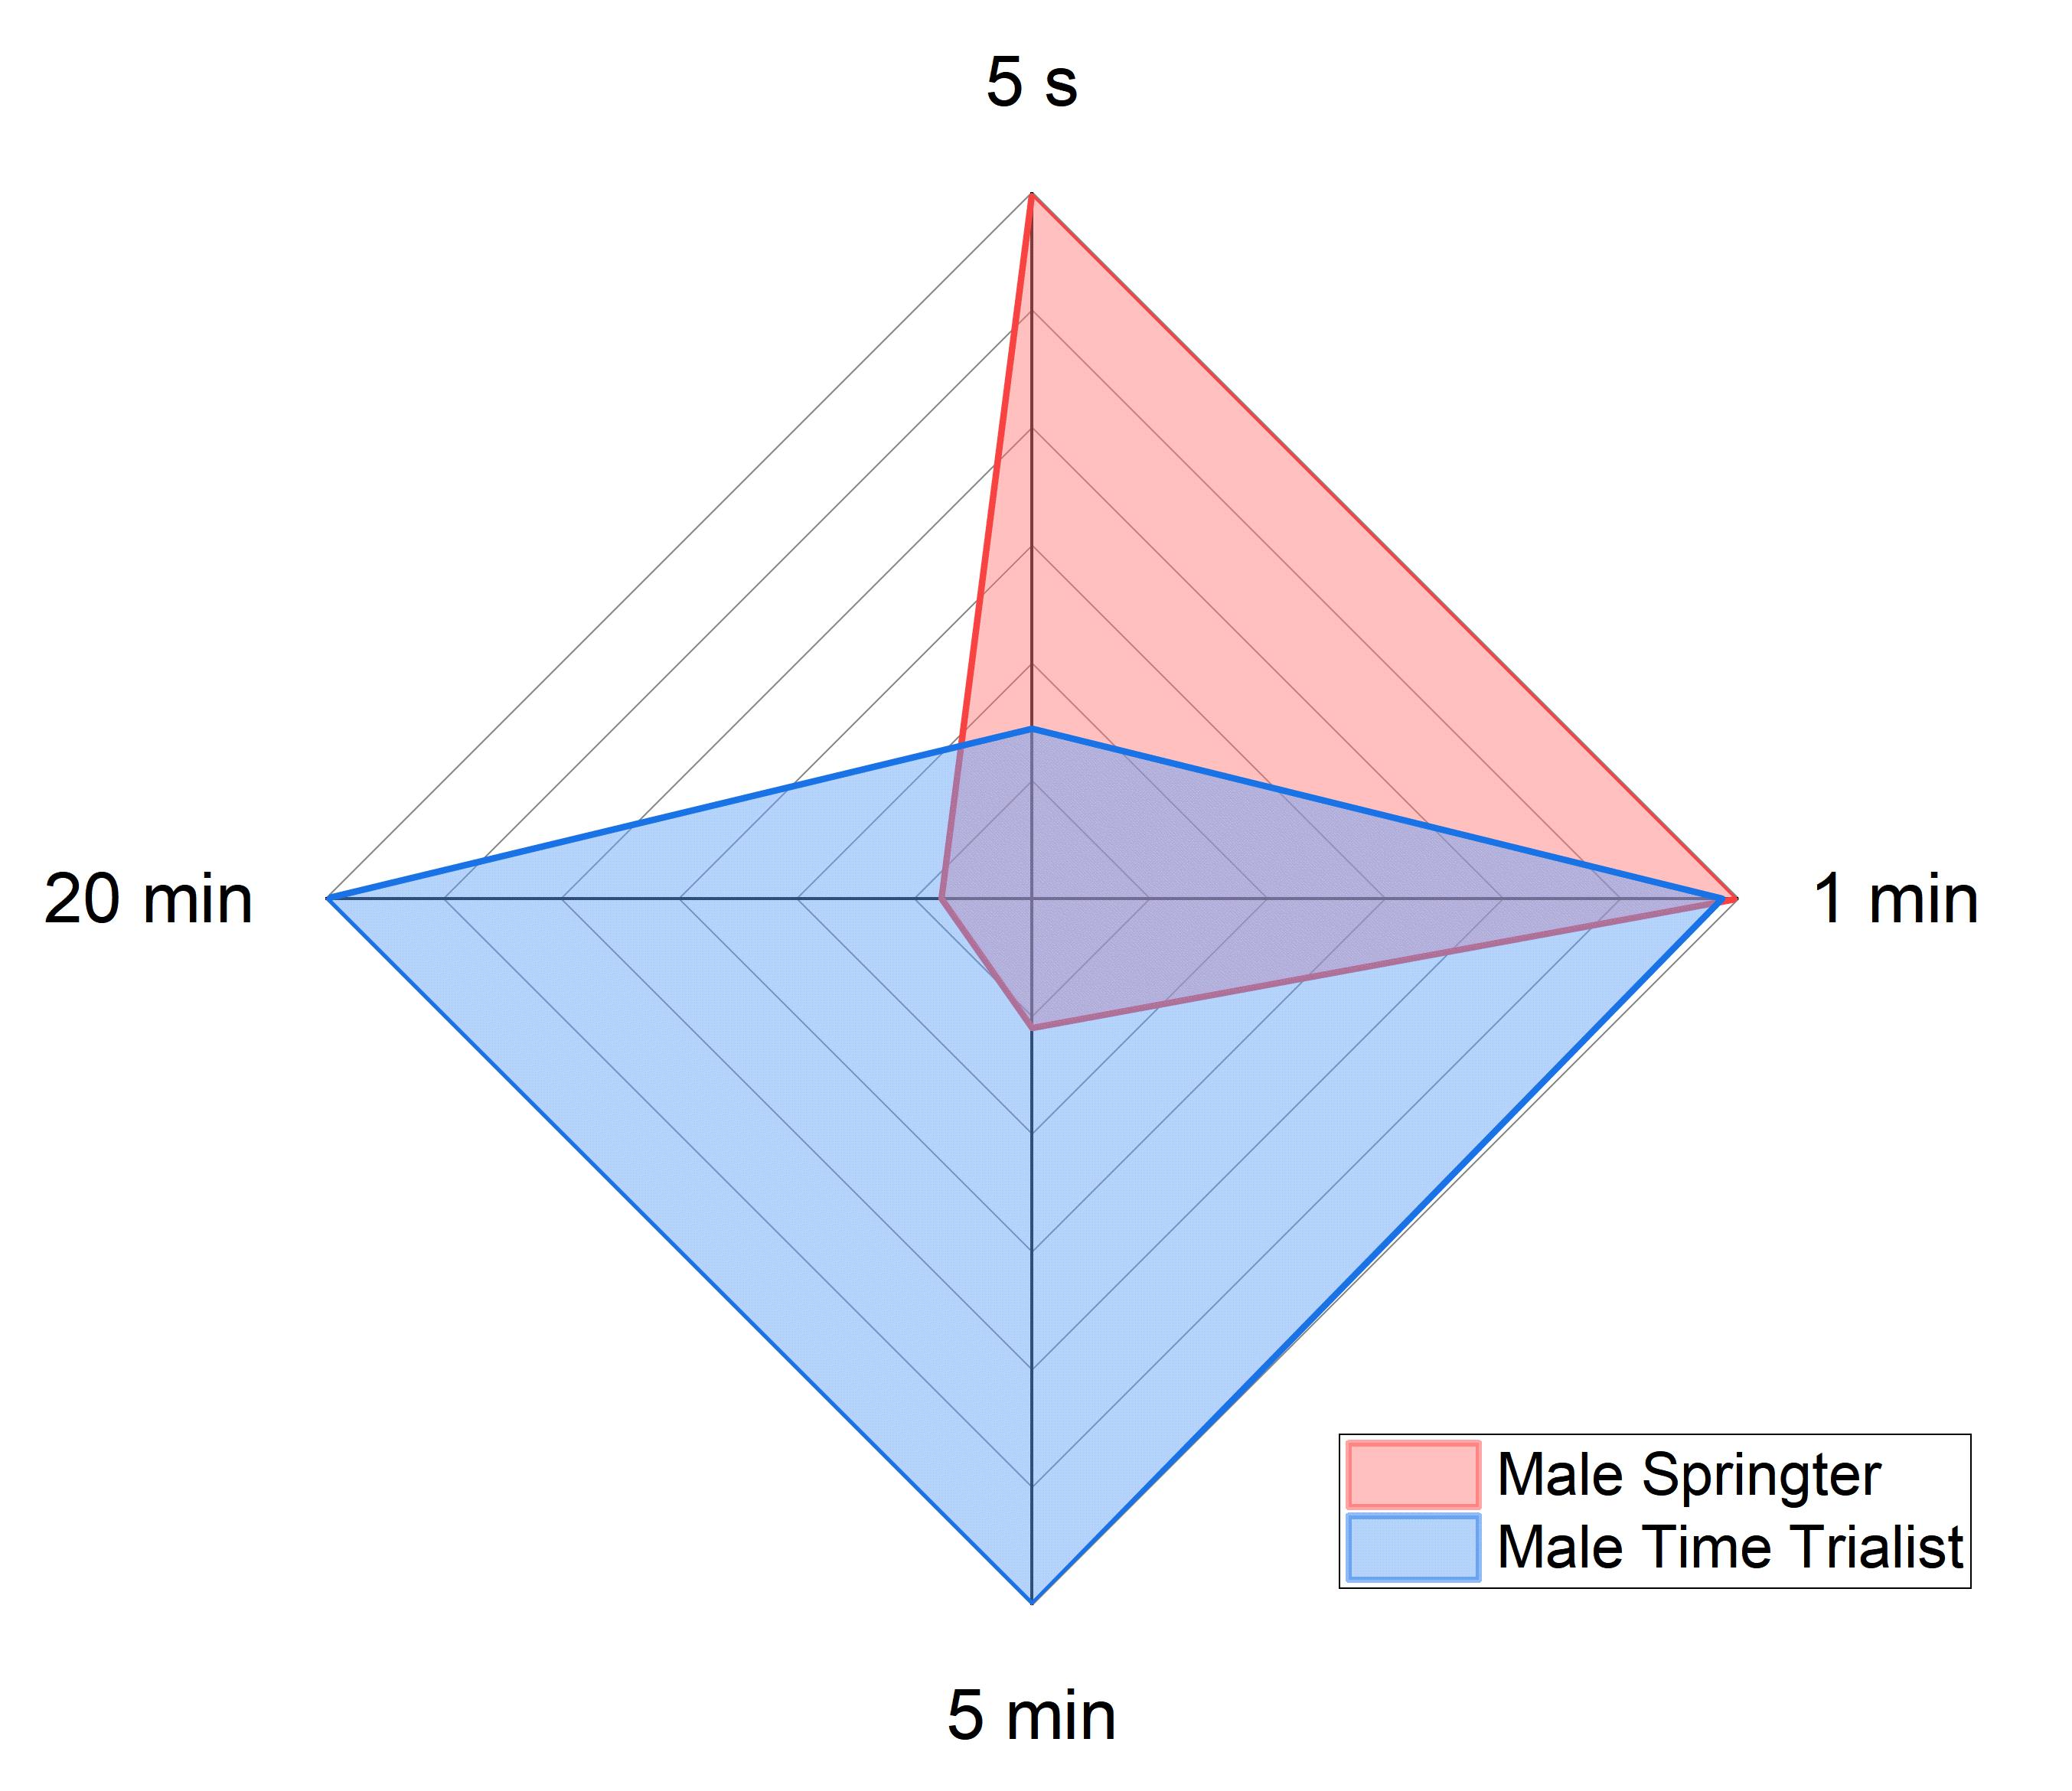
\includegraphics[width=0.7\linewidth]{image/radar/radar2}
		\caption{Radar map of male riders}
		\label{radar1}
	\end{minipage}
	\begin{minipage}[t]{0.45\textwidth}
		\centering
		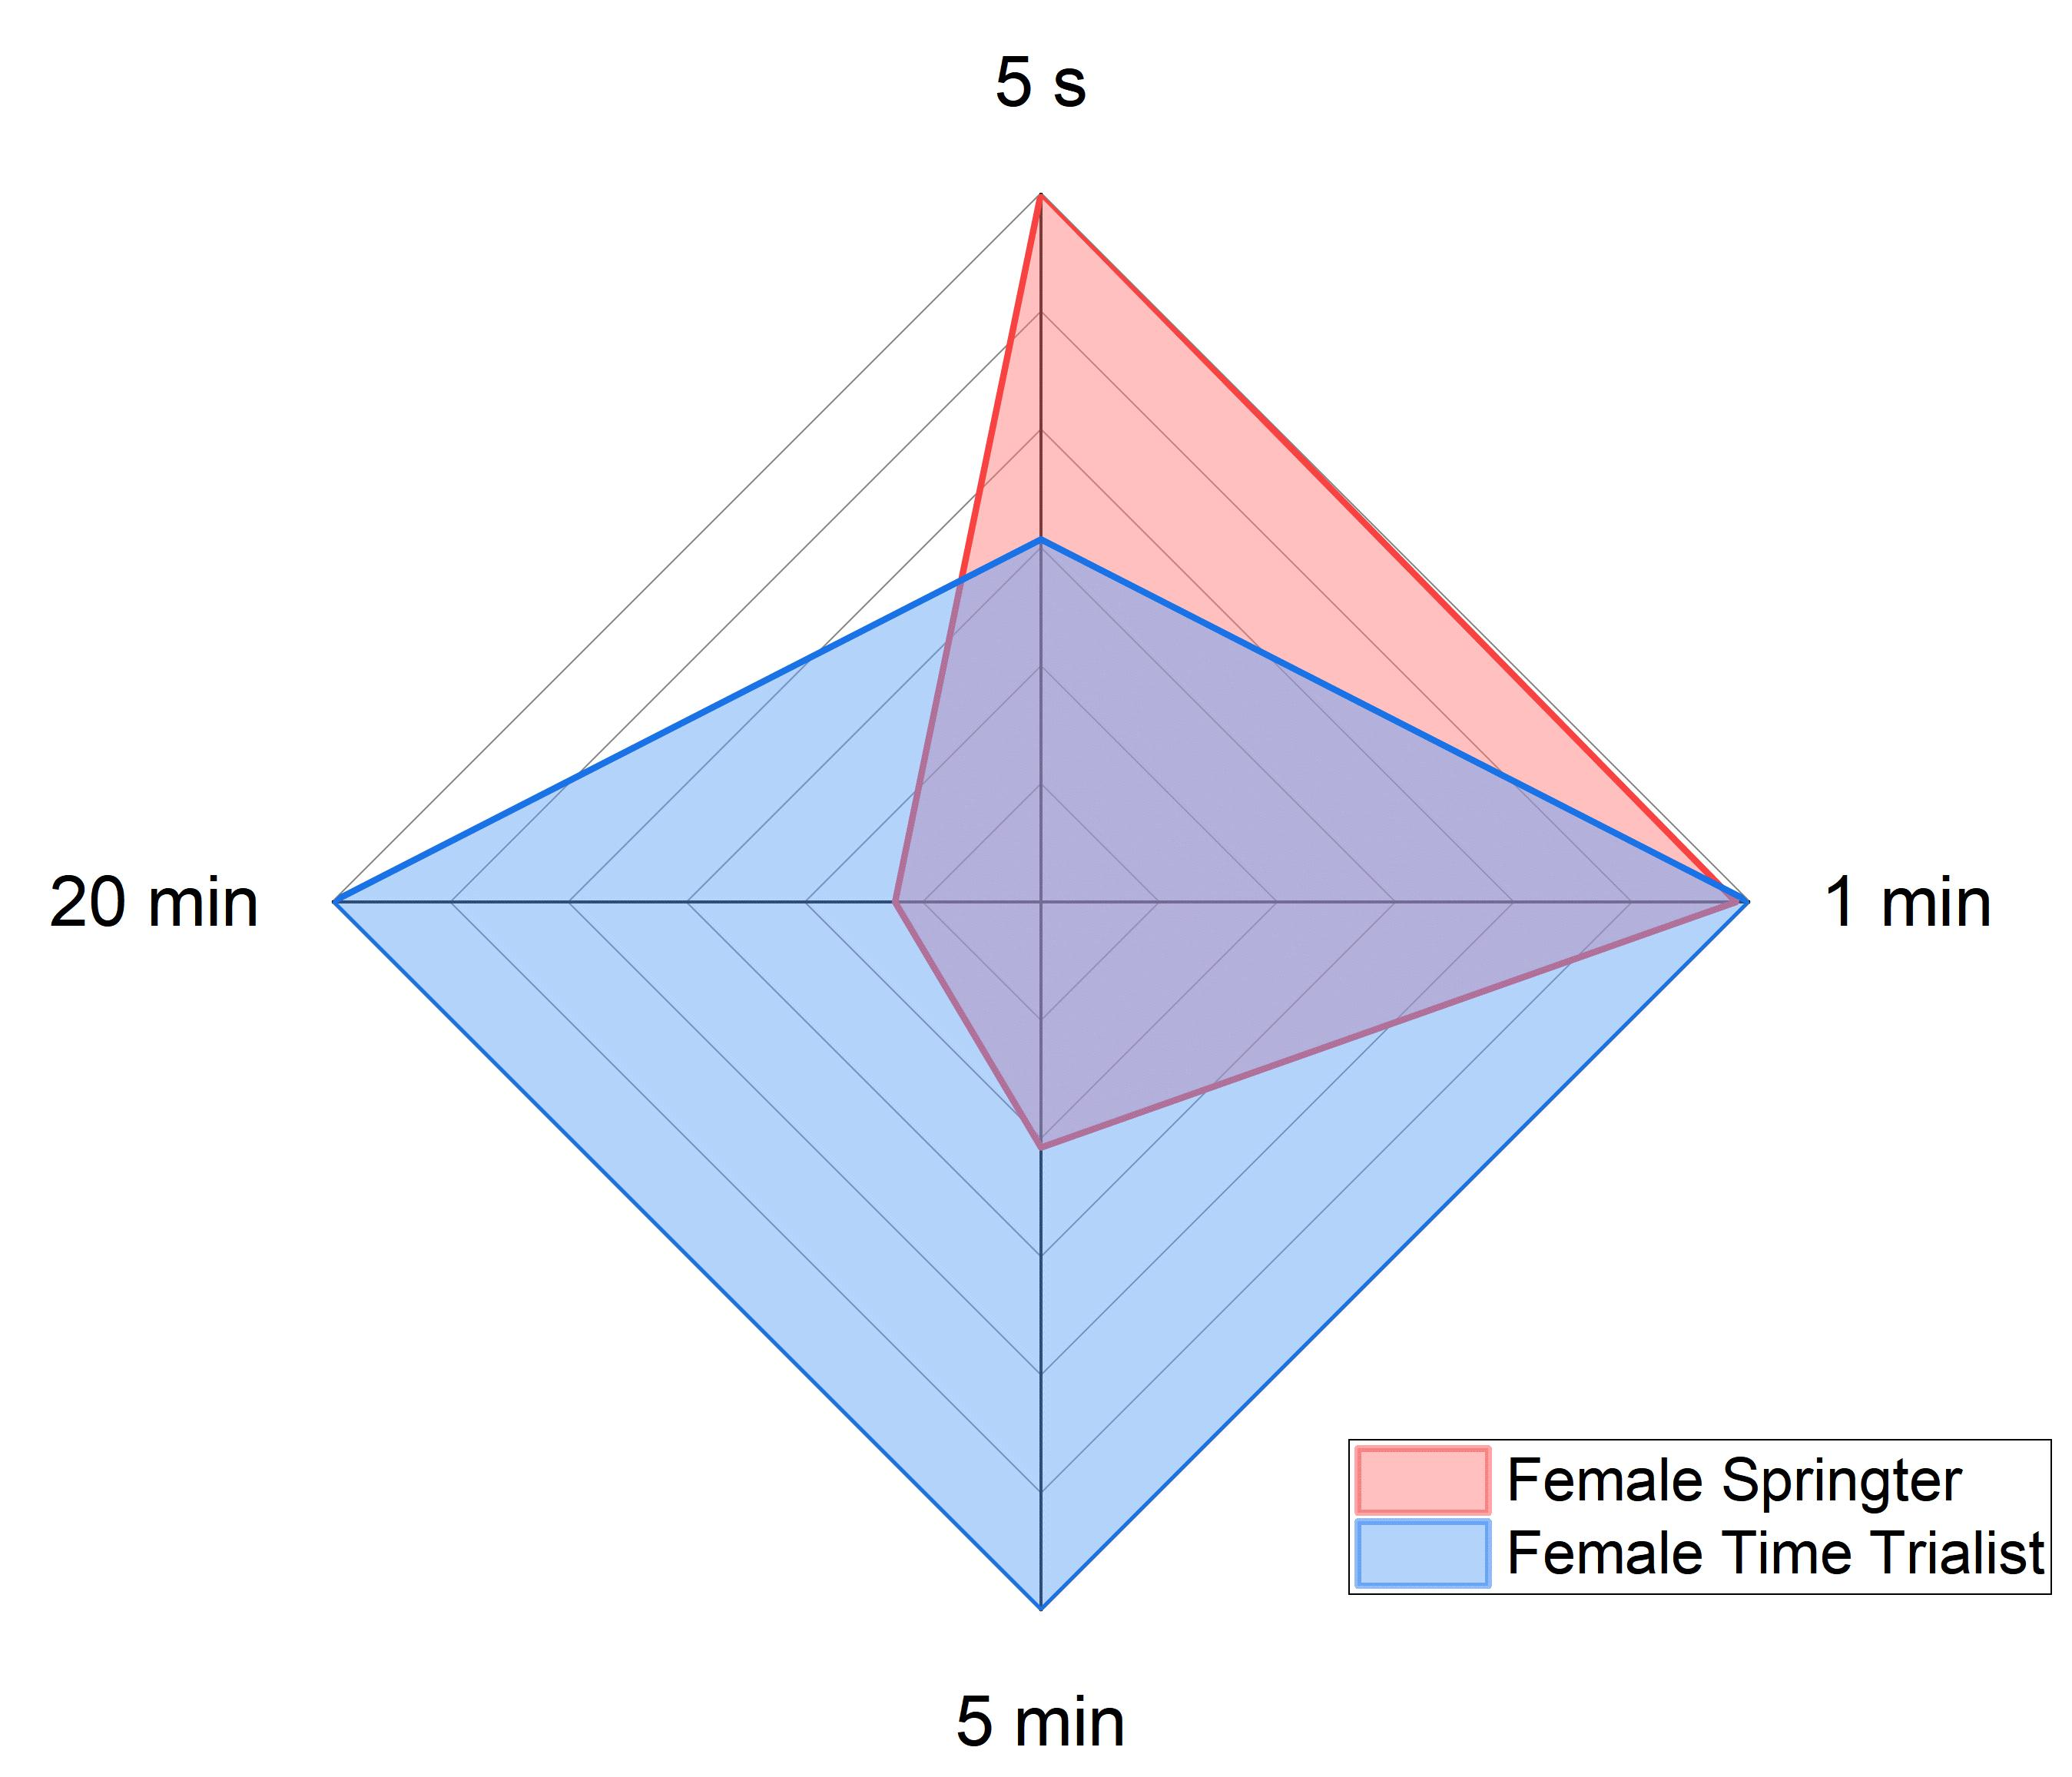
\includegraphics[width=0.7\linewidth]{image/radar/radar1}
		\caption{Radar map of female riders}
		\label{radar2}
	\end{minipage}
\end{figure}
\par As is shown in picture [\ref{radar1}][\ref{radar2}], sprinters  of both genders perform best in extreme intensity domain, while the two types of riders perform equally well in severe intensity domain. However, time trialists do much better in heavy and moderate domain.
\par With data from profile charts, we can sketch out the profile curve of different types of riders of different genders[\ref{sketch1}][\ref{sketch2}], and show their ability in four domains.
% TODO: \usepackage{graphicx} required
\begin{figure}[h]
	\centering
	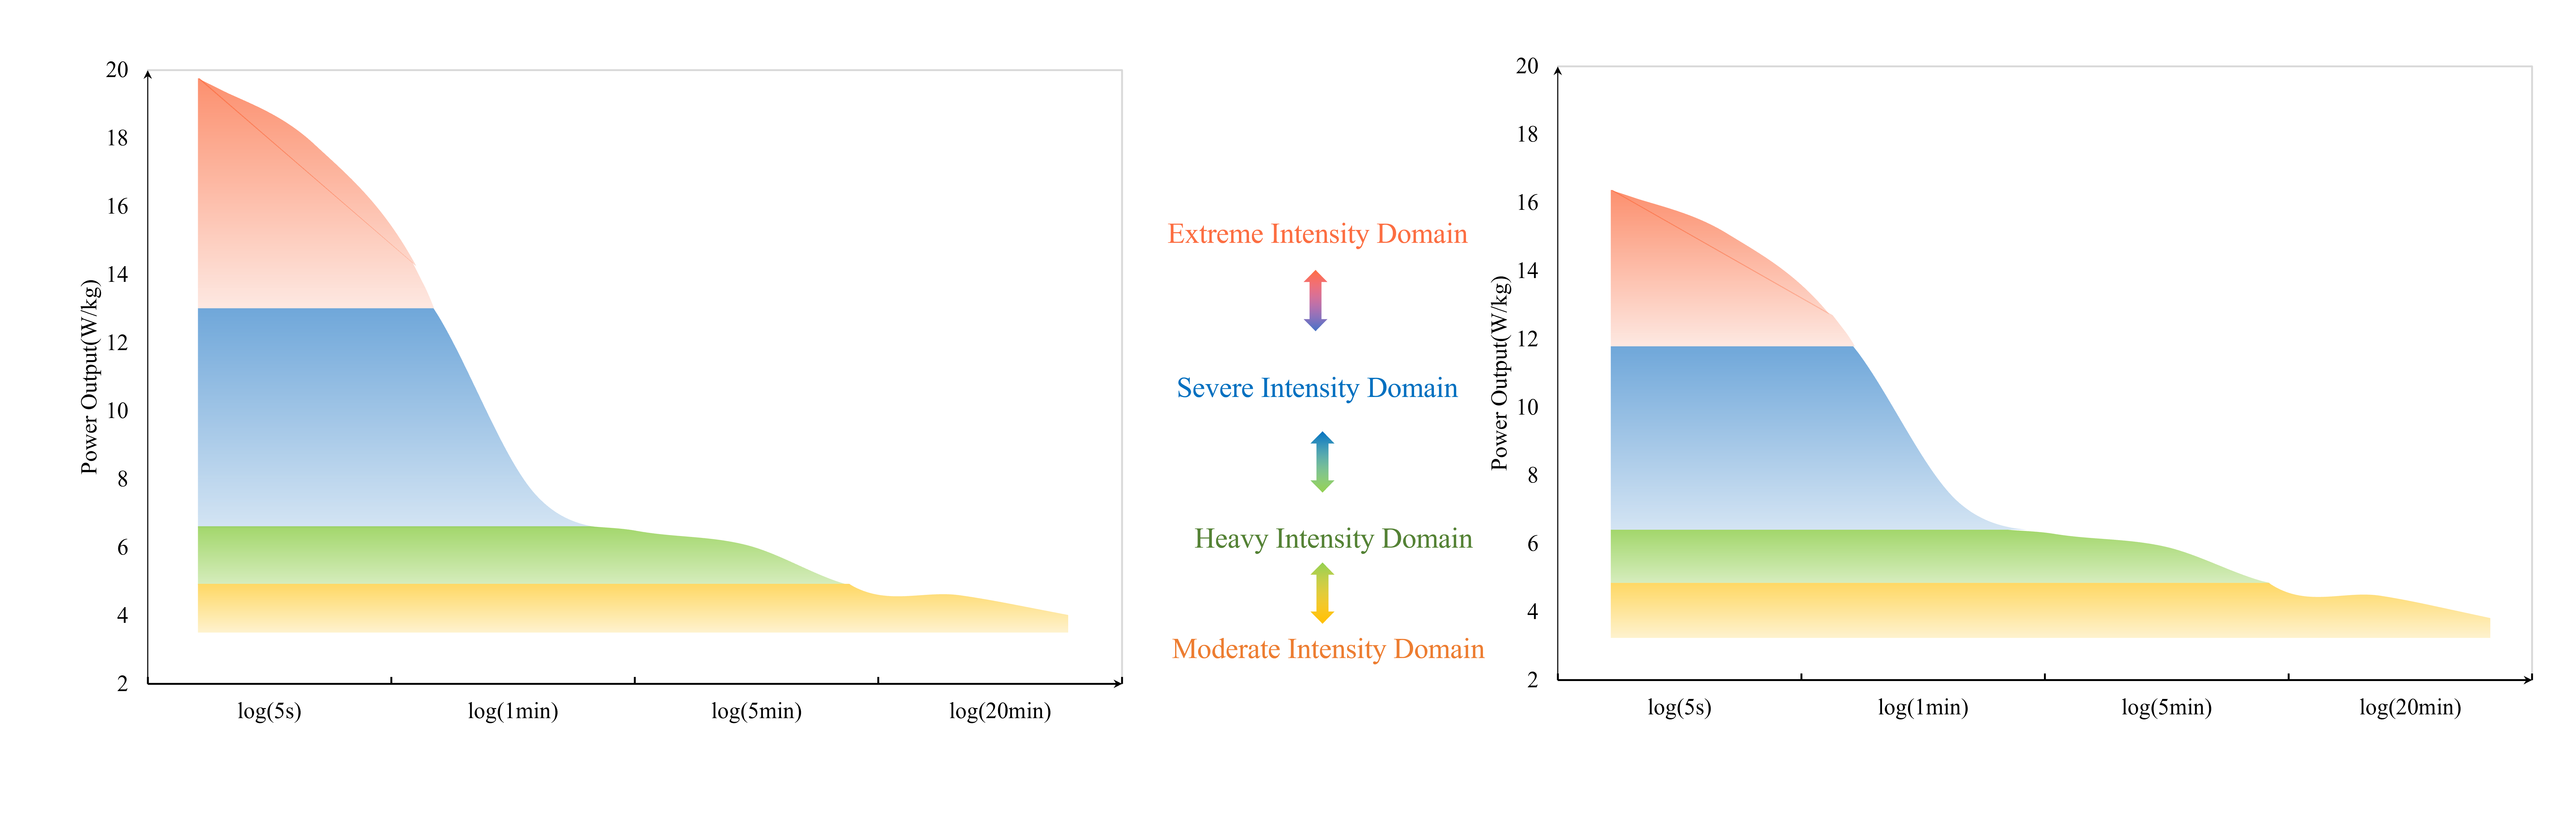
\includegraphics[width=1.0\linewidth]{image/sprinter}
	\caption{Sketch of power curve of male and female sprinters}
	\label{sketch1}
\end{figure}
% TODO: \usepackage{graphicx} required
\begin{figure}[h]
	\centering
	\includegraphics[width=1.0\linewidth]{"image/time trival"}
	\caption{Sketch of power curve of male and female time trialists}
	\label{sketch2}
\end{figure}

\par In order to reflect the distinction, we use the function to depict the relationship between power output per weight and time one man can maintain at that level:  
\begin{equation}
	\label{func}
	P=f(t)=at^b+c (b<0)
\end{equation}
The unknown parameters a and b represent different rider types and c represents different levels. For example, the function of sprinters have larger parameter of a and those who of world class have bigger c. In this sense, we name a and b as type parameter and c as level parameter.
\par In the next part, we will determine the value of parameters for functions of different rider types and genders to see whether the parameters will show how riders perform in different domains.
